\appendix

\section{In-Engine Windowed KV: Implementation}
\label{app:window}

\paragraph{Window half.} vLLM supports sliding-window attention for models that declare it: when a
decoder layer carries a \texttt{sliding\_window} attribute, the engine constructs a
\texttt{SlidingWindowSpec} for that layer's KV cache and the FlashAttention
backend~\citep{flashattn,flashattn2,flashinfer} applies a windowed causal mask. The KV manager then
frees blocks that fall entirely behind the window, which is what bounds resident memory --- the
property the collapse analysis of Section~\ref{sec:wall} turns on. Metronome sets
\texttt{sliding\_window}${=}W$ at model-construction time on the shared decoder-attention class that
the omni text backbones build, so every decoder layer reports a windowed spec; no scheduler,
allocator, or API change is required.

\paragraph{Sink half.} FlashAttention's window primitive cannot express the sink-anchored mask
$[0,S) \cup [t{-}W,t]$, so the sink half routes the decoder layers to vLLM's Triton unified-attention
backend and extends its kernel: the windowed mask gains the OR-term $k < S$, and the tile loop gains
$\lceil S/\mathrm{tile} \rceil$ extra leading iterations remapped onto the sink tiles --- the online
softmax is order-invariant, so accumulating them first is exact, and in segmented-decode mode only
segment~0 takes them, merged exactly once. On the memory side, the sliding-window KV manager pins each
request's first $\lceil S/\mathrm{block} \rceil$ blocks instead of freeing them, and the per-request
admission cap counts the pinned blocks so pool sizing stays exact. The kernel is verified against a
float32 reference of the union mask (mixed prefill/decode, grouped-query attention, both launch modes),
with freed blocks NaN-poisoned to prove nothing outside $\mathrm{sinks} \cup \mathrm{window}$ is ever
read; with $S{=}0$ every touched path is byte-identical to stock. The test ships with the artifact.

\section{Enabling Omni Streaming on Blackwell}
\label{app:fixes}

Running the omni models on vLLM~0.23 (the first release with resumable requests) on an SM120 Blackwell
GPU required four engine bug-fixes, without which the models do not initialize or stream; the combined
patch that ships with the artifact adds a fifth change, the in-engine bounded KV itself --- the sliding
window and its sink retention (Appendix~\ref{app:window}).

\begin{enumerate}[leftmargin=1.4em,itemsep=2pt]
\item \textbf{cu\_seqlens device.} The shared multimodal encoder attention builds \texttt{cu\_seqlens} on
the feature tensor's device (CPU during memory profiling) while q/k/v are on CUDA, crashing the varlen
flash-attention op~\citep{flashattn}. We coerce it to the query device.
\item \textbf{Capability gate.} FlashInfer~\citep{flashinfer} gates SM12.x support on the \emph{toolkit}
CUDA version. We gate on the \emph{runtime} version so Blackwell is recognized when the local
\texttt{nvcc} is older.
\item \textbf{JIT toolchain.} FlashInfer's bundled CCCL headers reject the CUDA-13.2 \texttt{nvcc}; the
documented escape macro (\texttt{CCCL\_DISABLE\_CTK\_COMPATIBILITY\_CHECK}) unblocks the JIT across a
CUDA minor version.
\item \textbf{mRoPE off-by-one.} A Qwen3-Omni position-id routine double-counts the audio start token,
overshooting the sequence length and crashing precisely when an audio block ends a streamed chunk --- the
per-frame append case. A one-line reconcile fixes it and is a no-op for every previously working input.
\end{enumerate}

With these, Qwen3-Omni-30B, Qwen2.5-Omni-7B, and MiniCPM-o-4.5 all load and stream; Moshi runs on its own
native stack. The evaluation also surfaced a sixth hazard: a resident streaming request that reaches
\texttt{max\_model\_len} does not stop cleanly --- the engine core crashes on a shape mismatch, killing
\emph{every} co-resident session at once. Unbounded per-session state is dangerous at more than one
boundary; our long-horizon runs size \texttt{max\_model\_len} above the session's growth to avoid it, and
Section~\ref{sec:discussion} argues the general fix is a first-class per-session state bound.

\section{Measurement Methodology: Fresh Worker Per Point}
\label{app:method}

Capacity curves for this workload must be measured with a freshly started worker per data point.
Measuring a capacity curve as a \emph{sweep} of many $N$ values on a single long-lived worker silently
inflates the apparent degradation at the larger $N$ values, which arrive later in the sweep: residual
engine state accumulates across points, and slowly varying ambient conditions (in our case, intermittent
contention from an unrelated GPU job) fold into whichever points run last. In our data this made the
unbounded baseline appear to collapse at $N{=}128$--$160$ in a 90\,s sweep, when a fresh worker per point
is flat to $N{=}160$ (Figure~\ref{fig:cliff}a), and it manufactured an apparent capacity cliff for Moshi
at $N{=}24$ that likewise vanished under fresh measurement. Every number in this paper is therefore
measured with one fresh worker per point. We recommend this as standard practice for interaction-serving
capacity measurement: the workload's long-lived resident state makes it unusually sensitive to
measurement-harness state.

\section{Additional Results}
\label{app:results}

\paragraph{Per-run wall outcomes.} Table~\ref{tab:wall} details the per-run outcomes behind
Figure~\ref{fig:cliff}b and \S\ref{sec:eval-cliff}: the fixed-order batch and the seeded
randomized-order replication (the shuffle and per-run logs ship with the artifact).

\begin{table}[h]
\centering\small
\caption{The latency cliff, per operating point (5 fresh runs each, 300\,s; bucket $p_{50}$). Unbounded
resident KV is a metastable gamble whose tip rate moves with the day's fill rate (\S\ref{sec:model});
in-engine windowed KV is flat in every run of both batches.}
\label{tab:wall}
\setlength{\tabcolsep}{4pt}
\begin{tabular}{lcc}
\toprule
& vanilla (unbounded KV) & in-engine windowed KV \\
\midrule
batch 1 (fixed order), $N{=}96$  & wall in $\mathbf{2/5}$ runs ($\rightarrow{\sim}1.6$\,s), else ${\sim}2$--$5$\,ms & ${\sim}1$--$2$\,ms, $\mathbf{0/5}$ wall \\
batch 1 (fixed order), $N{=}128$ & wall in $\mathbf{2/5}$ runs ($\rightarrow{\sim}1.6$\,s), else ${\sim}2$--$5$\,ms & ${\sim}2$--$12$\,ms, $\mathbf{0/5}$ wall \\
batch 2 (randomized), $N{=}96$   & wall in $\mathbf{5/5}$ runs ($\rightarrow{\sim}1.6$\,s) & flat few ms, $\mathbf{0/5}$ wall \\
batch 2 (randomized), $N{=}128$  & wall in $\mathbf{5/5}$ runs ($\rightarrow{\sim}1.6$\,s) & flat few ms, $\mathbf{0/5}$ wall \\
\bottomrule
\end{tabular}
\end{table}

\paragraph{In-engine windowing vs.\ application-level recycling.} Figure~\ref{fig:reencode} details the
comparison summarized in \S\ref{sec:eval-cliff}: three policies with the same memory horizon.

\begin{figure}[h]
\centering
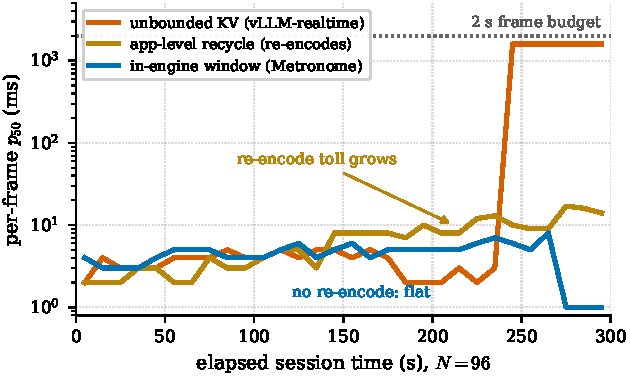
\includegraphics[width=0.62\linewidth]{figures/reencode.pdf}
\caption{\textbf{In-engine windowing beats application-level recycling.} Three policies with the same
memory horizon at $N{=}96$ over 300\,s (per-frame $p_{50}$, 10\,s buckets). Unbounded resident KV hits
the wall at ${\sim}240$\,s. The application-level recycling proxy avoids the wall but its periodic
re-encode grows over the call ($p_{50}$ to ${\sim}14$--$17$\,ms, $p_{90}$ to $36$\,ms). The in-engine
window bounds the horizon without ever re-encoding.}
\label{fig:reencode}
\end{figure}

\paragraph{Window-size ablation.} Figure~\ref{fig:wabl} sweeps the window size at fixed load. Latency is
flat up to a 2048-token (${\sim}80$\,s) window; the lone $p_{90}$ uptick at 4096 tokens carries a
$p_{99}$ comparable to the smaller windows', so we attribute it to single-run tail noise rather than a
clean attention effect. A memory horizon well beyond the ${\sim}30$\,s most interactions need is free.

\begin{figure}[h]
\centering
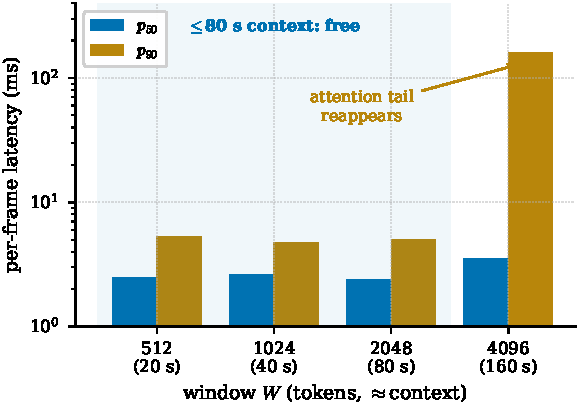
\includegraphics[width=0.6\linewidth]{figures/window_ablation.pdf}
\caption{\textbf{A generous window is free.} Window-size ablation (in-engine windowed KV, $N{=}128$,
60\,s runs): $p_{50}/p_{90}$ stay ${\sim}5$\,ms up to a 2048-token (${\sim}80$\,s) window.}
\label{fig:wabl}
\end{figure}

\paragraph{Turn-based quality detail.} In the turn-based probe of Section~\ref{sec:quality} ($N{=}96$,
75\,s sessions, EOS-terminated turns), answer-stated counts are $96/96$ sessions for both vanilla and
windowed policies, with per-frame correctness ${\sim}70\%$ vs.\ ${\sim}68\%$ (statistically
indistinguishable). The gap from $100\%$ per-frame is genuine model behavior on looped, sometimes
partial audio and is identical across policies.

\paragraph{Free-running conditions: sweep and boundary controls.} Table~\ref{tab:sinksweep} collects
every free-running condition --- the ablation of Figure~\ref{fig:longhz} plus the sink/window sweep,
with boundary controls at the exact token-layout edges. The controls localize the harm of
over-pinning (\S\ref{sec:quality}): a pin that \emph{truncates} the first audio block is harmless
($S{=}32$), refuting the malformed-block hypothesis, and the failure signatures in the outcome column
track how much first-turn \emph{content} the pin keeps semantically live. Engine-side, the rows
differ only as block arithmetic dictates (pool column: plateau $\propto W$, plus ${\sim}0.1\%$ of the
pool per pinned sink block) and latency is flat in every run, so the quality differences are entirely
model behavior. The unbounded baseline's pool was still climbing when its 300\,s session ended --- at
$N{=}32$ the session outlives the run, the benign side of the two-clock race of \S\ref{sec:model}.

\begin{table}[h]
\centering\small
\caption{All free-running probe conditions (Figure~\ref{fig:longhz} and the sink/window sweep;
$N{=}32$, 300\,s, one fresh worker per row, per-frame $p_{99}{\le}3$\,ms and zero errors throughout).
\emph{Mid-call}: sessions answering the currently playing question over ages 30--240\,s.
\emph{Fresh Q}: the synthesized-voice question at 240--270\,s. \emph{Pool}: KV-pool occupancy
plateau. Token layout: chat header $[0,14)$, first audio $[14,42)$, instruction $[42,53)$,
assistant-open $[53,58)$, generated from $58$.}
\label{tab:sinksweep}
\footnotesize
\setlength{\tabcolsep}{4pt}
\begin{tabular}{llcccl}
\toprule
$(W,\,S)$ & pin covers & mid-call & fresh Q & pool & outcome \\
\midrule
unbounded      & ---                              & $23$--$27\%$ & $26\%$ & $74\%\,\uparrow$ & steady; pool still filling at 300\,s \\
\midrule
$(512,\,0)$    & --- (sinks ablated)              & $\to 3\%$    & $7\%$  & $3.3\%$  & decays as window slides \\
$(1024,\,0)$   & --- (sinks ablated)              & $\to 0$--$8\%$ & $6\%$ & $6.4\%$  & decays \\
$(2048,\,0)$   & --- (sinks ablated)              & $\to 0\%$    & $0\%$  & $12.7\%$ & decays \\
$(1024,\,0)$   & --- (sink kernel, control)       & $\to 0\%$    & $0\%$  & $6.5\%$  & decays: kernel is not the cause \\
\midrule
$(1024,\,16)$  & chat header                      & $38$--$57\%$ & $45\%$ & $6.5\%$  & \textbf{recovers --- best} \\
$(1024,\,32)$  & $+\,{\sim}2/3$ of first audio    & $33$--$45\%$ & $21\%$ & $6.5\%$  & recovers \\
$(1024,\,42)$  & $+$ complete first audio         & $20$--$32\%$ & $21\%$ & $6.6\%$  & degraded: answers the pinned clip \\
$(1024,\,58)$  & $+$ instruction, assistant-open  & $25$--$37\%$ & $18\%$ & $6.8\%$  & degraded: quotes the pinned clip \\
$(1024,\,64)$  & $+$ first 6 \emph{generated} tokens & $\to 7\%$ & $8\%$  & $6.6\%$  & collapses: template echo \\
\midrule
$(512,\,32)$   & as $(1024,32)$                   & $\to 0\%$    & $0\%$  & $3.5\%$  & too-small window; sinks no rescue \\
$(2048,\,32)$  & as $(1024,32)$                   & $40$--$57\%$ & $42\%$ & $12.8\%$ & recovers; matches $W{=}1024$ \\
\bottomrule
\end{tabular}
\end{table}
